\documentclass{report}
\usepackage{graphicx}
\usepackage[frame,line,arrow,matrix,tips]{xy}	% all that is usually necessary
\title {\author{ Josh Rendon, Micah Thornton} Proposal for Quantum Reversible Synthesis}

\begin{document}
\maketitle{}
\begin{abstract}
\end{abstract}
\section{problem definition}
There are a number of classical circuits that benefit from the property of being a mathematical bijection. For instance a hash function necessarily needs
to be a mathematical bijection in order to ensure there are no collisions in the mapping from inputs to hash outputs. 
Unfortunately, <computationally efficient> methods do not currently exist to determine if a circuit is in fact a bijection.
We propose the implementation of a software synthesis tool based on current work in the literature to determine if a classical circuit is a mathematical bijection.
If this circuit is synthesizable as a quantum cascade with no garbage outputs and no ancillia inputs then we know the circuit is logically reversible and is a bijection.
\section{ }
% 
% File: 4-bit_circular_hash_qc.qasm
% Date: March 21 2015
% Authors: Josh Rendon, Micah Thornton
%
%  def not,0,'$\oplus$'
%  def toffoli4,3,'$\oplus$'
% 
%  qubit in4
%  qubit in3
%  qubit in2
%  qubit in1
% 
%  toffoli4      in4,in3,in2,in1
%  toffoli       in4,in3,in2
%  cnot          in4,in3
%  not           in4

%  Time 01:
%    Gate 00 toffoli4(in4,in3,in2,in1)
%  Time 02:
%    Gate 01 toffoli(in4,in3,in2)
%  Time 03:
%    Gate 02 cnot(in4,in3)
%  Time 04:
%    Gate 03 not(in4)

% Qubit circuit matrix:
%
% in4: gAxA, gBxA, gCxA, gDxA, n  
% in3: gAxB, gBxB, gCxB, n  , n  
% in2: gAxC, gBxC, n  , n  , n  
% in1: gAxD, n  , n  , n  , n  

\documentclass[11pt]{article}
%
% File:   xyqcirc.tex
% Date:   14-Mar-04
% Author: I. Chuang <ichuang@mit.edu>
%
% Definitions for producing quantum circuits with XYPIC in latex
%
% $Log: xyqcirc.tex,v $
% Revision 1.17  2004/03/25 05:01:23  ike
% discard and slash
%
% Revision 1.16  2004/03/25 04:58:42  ike
% added discard, and variable width dmeter
%
% Revision 1.15  2004/03/24 23:43:33  ike
% \dmeter and \sq
%
% Revision 1.14  2004/03/24 20:29:40  ike
% added \t for swap
%
% Revision 1.13  2004/03/24 17:52:16  ike
% removed \w from \gspace
%
% Revision 1.12  2004/03/24 16:38:34  ike
% added small space before |0> for \z
%
% Revision 1.11  2004/03/24 16:23:11  ike
% added \z
%
% Revision 1.10  2004/03/24 16:19:11  ike
% added multiple qubit operations
%
% Revision 1.9  2004/03/24 03:03:44  ike
% typo
%
% Revision 1.8  2004/03/24 02:50:09  ike
% added qv
%
% Revision 1.7  2004/03/24 00:07:34  ike
% add \m matrix op
%
% Revision 1.6  2004/03/23 23:13:10  ike
% misc
%
% Revision 1.5  2004/03/23 23:12:42  ike
% works now
%
% Revision 1.4  2004/03/23 22:22:34  ike
% ifthen also failes - because xymatrix entries in \save...\restore
%
% Revision 1.3  2004/03/23 21:34:36  ike
% no q/c wire switching
%
% Revision 1.2  2004/03/23 21:25:29  ike
% classical qo quantum wire switching try
%
% Revision 1.1  2004/03/23 21:01:46  ike
% Initial revision
%

%%%%%%%%%%%%%%%%%%%%%%%%%%%%%%%%%%%%%%%%%%%%%%%%%%%%%%%%%%%%%%%%%%%%%%%%%%%%%
% preliminaries

\usepackage{graphicx}

\usepackage[frame,line,arrow,matrix,tips]{xy}	% all that is usually necessary
\CompilePrefix{xygui-}
\makeindex
\pagestyle{empty}

\setlength{\oddsidemargin}{-0.5in}	% 1.25in left margin 
\setlength{\evensidemargin}{-0.5in}	% 1.25in left margin (even pages)

\setlength{\topmargin}{0.0in}		% 1in top margin
\setlength{\textwidth}{6.25in}		% 6.0in text - 1.25in rt margin
\setlength{\textheight}{8.6in}		% Body ht for 1in margins
\addtolength{\topmargin}{-\headheight}	% No header, so compensate
\addtolength{\topmargin}{-\headsep}	% for header height and separation

\begin{document}

\thispagestyle{empty}

%%%%%%%%%%%%%%%%%%%%%%%%%%%%%%%%%%%%%%%%%%%%%%%%%%%%%%%%%%%%%%%%%%%%%%%%%%%%%
% wires

\def\w{\ar@{-}[l]}
\def\W{\ar@{=}[l]}

%%%%%%%%%%%%%%%%%%%%%%%%%%%%%%%%%%%%%%%%%%%%%%%%%%%%%%%%%%%%%%%%%%%%%%%%%%%%%
% labels

% simple label
\def\A#1{\save []="#1" \restore}

%%%%%%%%%%%%%%%%%%%%%%%%%%%%%%%%%%%%%%%%%%%%%%%%%%%%%%%%%%%%%%%%%%%%%%%%%%%%%
% single qubit operations

\def\op#1{*+[F]{\rule[-0.2ex]{0ex}{2.1ex}#1}}	% operator in box
\def\b{*={\bullet}}
\def\o{*={\oplus}}
\def\t{*={\times}}				% for swap gate
\def\sq{*=<6pt,6pt>[F]{}}			% square, for controlled-phase
\def\m#1{\left[\matrix{#1}\right]}		% matrix shortcut
\def\z{*+[]{\rule[-0.2ex]{0ex}{2.1ex}~|0\>}}	% re-init to |0>
\def\discard{*[]{\rule[-0.2ex]{0.75pt}{2.1ex}~}}	% vertical ``|''
\def\slash{*={/}}				% slash for wire bundles

%%%%%%%%%%%%%%%%%%%%%%%%%%%%%%%%%%%%%%%%%%%%%%%%%%%%%%%%%%%%%%%%%%%%%%%%%%%%%
% nop's

\def\N{*-{}\W}
\def\n{*-{}\w}

%%%%%%%%%%%%%%%%%%%%%%%%%%%%%%%%%%%%%%%%%%%%%%%%%%%%%%%%%%%%%%%%%%%%%%%%%%%%%
% misc definitions

\def\>{\rangle}
\def\<{\langle}
\def\ua{\uparrow}

% measurement box
\def\meter{*+[]{\put(-3,0){\includegraphics[scale=.5]{meter.epsf}}~~~~}%
		\ar@{-}[l]}

%%%%%%%%%%%%%%%%%%%%%%%%%%%%%%%%%%%%%%%%%%%%%%%%%%%%%%%%%%%%%%%%%%%%%%%%%%%%%
% qubit names (and also revert to qubit wires, vs, cbit wires)

\def\q#1{*+{\rule[-0.2ex]{0ex}{2.1ex}|#1\>}}
\def\qv#1#2{*+{\rule[-0.2ex]{0ex}{2.1ex}|#1\>=|#2\>}}
	
%%%%%%%%%%%%%%%%%%%%%%%%%%%%%%%%%%%%%%%%%%%%%%%%%%%%%%%%%%%%%%%%%%%%%%%%%%%%%
% multiple qubit gates

% utulity text box for figuring out width of things
\newbox{\sbox}

% empty space of width determined by the text argument
\def\gspace#1{*+{\rule[-0.2ex]{0ex}{2.1ex}%
	\setbox\sbox=\hbox{$#1$}%
	\hspace*{\wd\sbox}}}
	
% n-qubit operation #1=box label, #2=number of qubits (eg d=2 qubits, ddd=4)
\def\gnqubit#1#2{\gspace{#1}
		 \save [].[#2]!C="qq"*[F]\frm{}\restore
		 \save "qq"*[]{#1} \restore}

% two-qubit operation
\def\gtwo#1{\gnqubit{#1}{d}}

% two-qubit operation
\def\gthree#1{\gnqubit{#1}{dd}}

%%%%%%%%%%%%%%%%%%%%%%%%%%%%%%%%%%%%%%%%%%%%%%%%%%%%%%%%%%%%%%%%%%%%%%%%%%%%%
% ``D'' style measurement gate a-la-cleve, at Michael Nielsen's request

\def\dmeterwide#1#2{*{\xy <0pt,-8pt>;<0pt,8pt> **@{-};
		    <0pt,-8pt>;<#2,-8pt> **@{-} ;
		    <0pt, 8pt>;<#2, 8pt> **@{-} ;
		    <#2,0pt>-<5pt,0pt>*{#1} ;
		    <#2,0pt>*\cir<8pt>{r_l}\endxy}}

\def\dmeter#1{\dmeterwide{#1}{12pt}}

%%%%%%%%%%%%%%%%%%%%%%%%%%%%%%%%%%%%%%%%%%%%%%%%%%%%%%%%%%%%%%%%%%%%%%%%%%%%%


% definitions for the circuit elements

\def\gAxA{\b\w\A{gAxA}}
\def\gAxB{\b\w\A{gAxB}}
\def\gAxC{\b\w\A{gAxC}}
\def\gAxD{\op{$\oplus$}\w\A{gAxD}}
\def\gBxA{\b\w\A{gBxA}}
\def\gBxB{\b\w\A{gBxB}}
\def\gBxC{\o\w\A{gBxC}}
\def\gCxA{\b\w\A{gCxA}}
\def\gCxB{\o\w\A{gCxB}}
\def\gDxA{\op{$\oplus$}\w\A{gDxA}}

% definitions for bit labels and initial states

\def\bA{ \q{in_{4}}}
\def\bB{ \q{in_{3}}}
\def\bC{ \q{in_{2}}}
\def\bD{ \q{in_{1}}}

% The quantum circuit as an xymatrix

\xymatrix@R=5pt@C=10pt{
    \bA & \gAxA &\gBxA &\gCxA &\gDxA &\n  
\\  \bB & \gAxB &\gBxB &\gCxB &\n   &\n  
\\  \bC & \gAxC &\gBxC &\n   &\n   &\n  
\\  \bD & \gAxD &\n   &\n   &\n   &\n  
%
% Vertical lines and other post-xymatrix latex
%
\ar@{-}"gAxD";"gAxA"\ar@{-}"gAxD";"gAxB"\ar@{-}"gAxD";"gAxC"
\ar@{-}"gBxC";"gBxA"\ar@{-}"gBxC";"gBxB"
\ar@{-}"gCxB";"gCxA"
}

\end{document}

\begin{figure}
  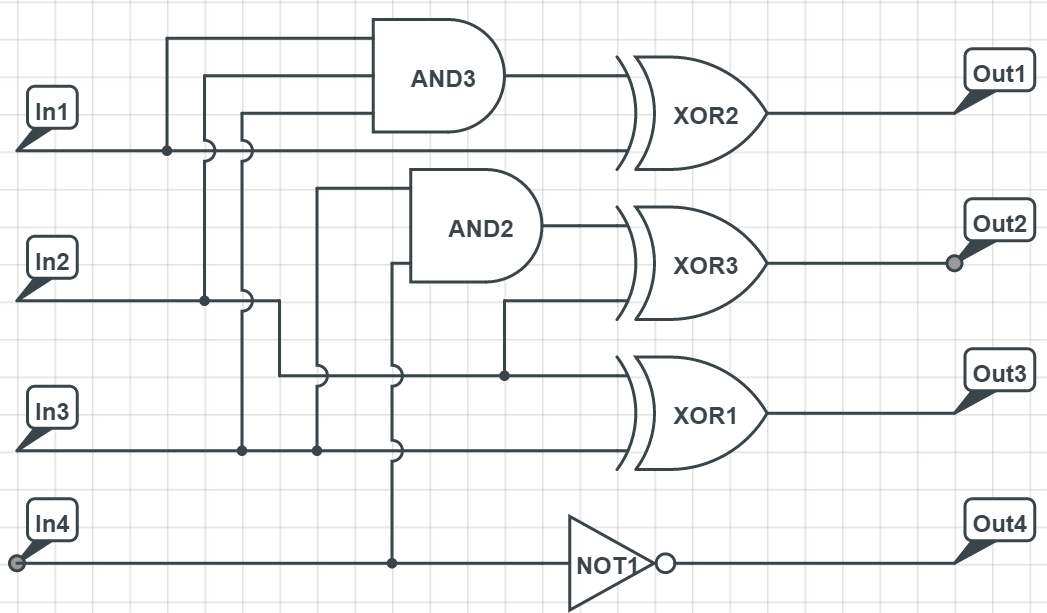
\includegraphics{figures/4-bit_circular_hash_schematic.PNG}
\end{figure}

\end{document}
